\section{Aufbau}
\label{sec:Aufbau}
Es wird eine Schaltung gemäß des in Abbildung \ref{fig:Aufbau} zu sehenden Schemas aufgebaut. Die als Probe verwendete $\beta$-Quelle wird auf der Seite des eingewölbten Fensters aus Mylarfolie positioniert. Zwischen Anodendraht und Zylindermantel wird die Spannung $U$ angelegt. Die durch die Strahlung an der Anode entstehende Ladung kann über den Widerstand $R$ abfließen, wodurch ein Spannungsimpuls entsteht. Dieser wird vom Kondensator entkoppelt und kann über einen Verstärker vom Zähler gemessen und vom Oszilloskop dargestellt werden.
\begin{figure}
\centering
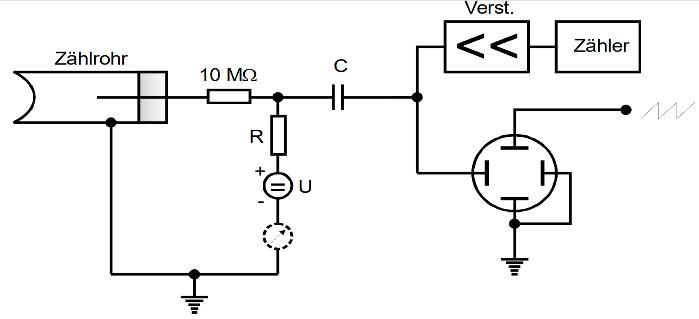
\includegraphics[scale=0.5]{content/images/aufbau2.jpg}
\caption{Versuchsaufbau zur Bestimmung der Kenndaten eines Geiger-Müller-Zählrohrs \cite{V703}.}
\label{fig:Aufbau}
\end{figure}